\chapter{A rendelések adatainak nyilvántartása}

Itt magáról az adatmodellről van szó gyakorlatilag. Itt érdemes kifejteni, hogy milyen adat, és hol kerül majd tárolásra. Az ER jellegű diagram, illetve az SQLAlchemy-s modellek egyszerűsített változata kellene majd ide.

A rendelések adatainak nyilvántartása
Az adatbázis tervezése során az egyik fő célom az volt, hogy könnyen módosítható, illetve kibővíthető legyen a rendszer. Első lépésként a fontosabb egyedeket határoztam meg, majd a köztük lévő kapcsolatokat. A dolgozatom készítése során elkészítettem két kezdetleges adatmodellt, amelyeknek az összefésüléséből megszületett a végleges adatmodell. Az alkalmazás implementálása során számos alkalommal kellett módosítanom az adatbázist.

Az általam tervezett adatmodell egyes táblái és a köztük lévő kapcsolatok \aref{fig:rendeles_sema} ábrán láthatók.

\begin{figure}
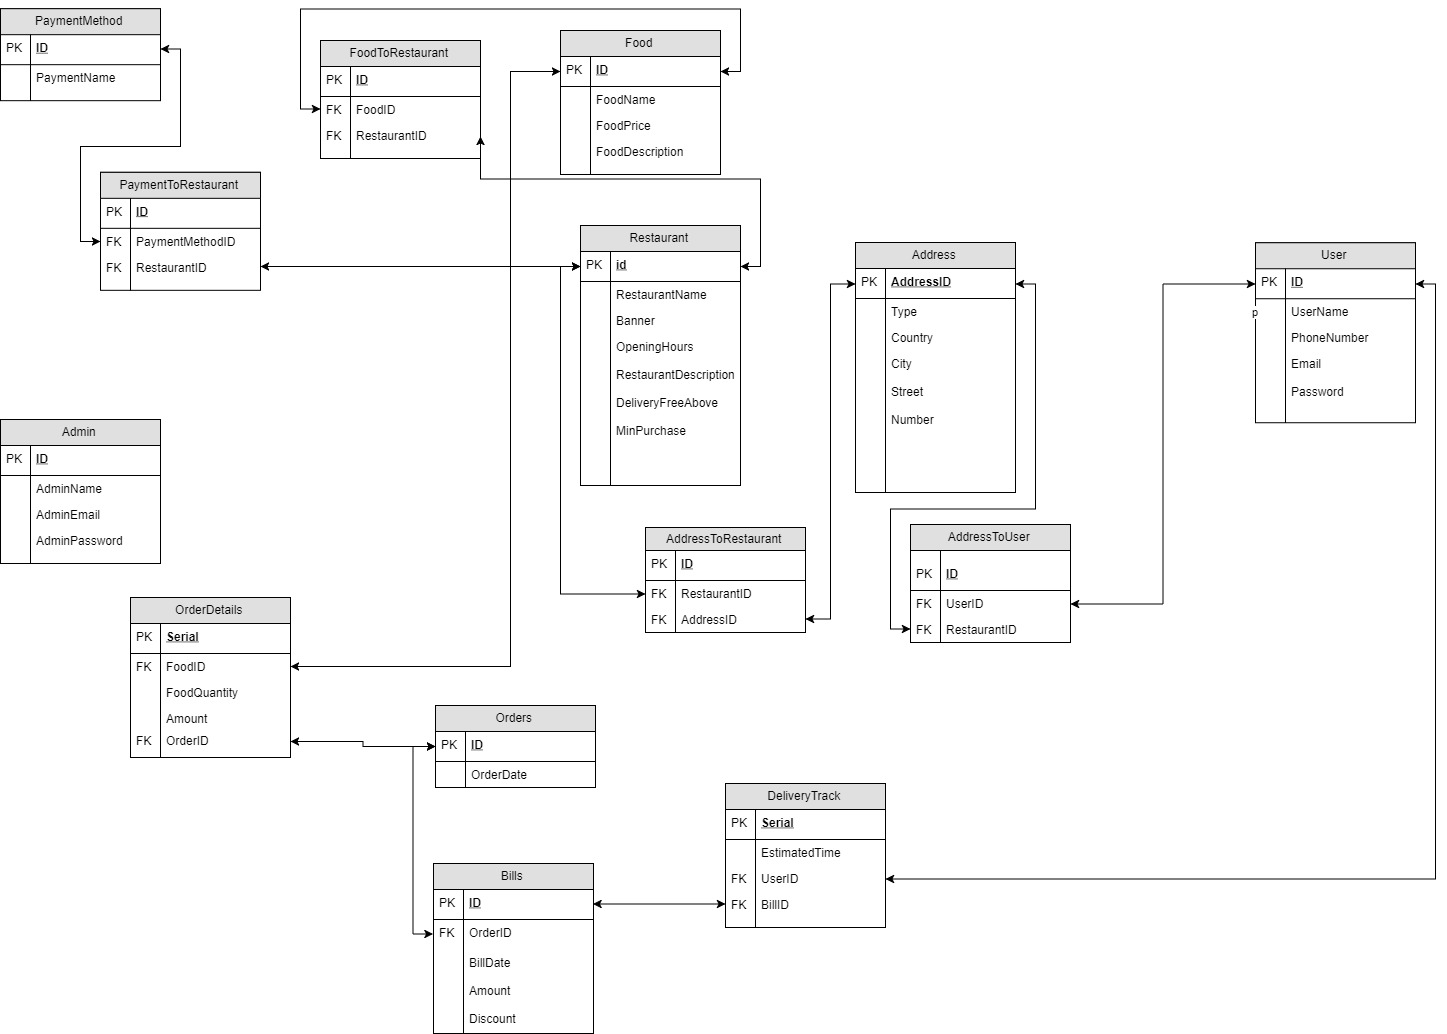
\includegraphics[scale=0.3]{kepek/rendeles_sema.jpg}
\caption{A rendelések adatait kezelő adatábis sémája}
\label{fig:rendeles_sema}
\end{figure}

\section{users}

Az online alkalmazásomon keresztül való étel rendeléshez regisztrált felhasználónak kell lenni. Ez a tábla a regisztrált felhasználókról tartalmaz információkat, illetve az adatbázisban lévő éttermek tulajdonosairól. Minden felhasználó rendelkezik egy azonosítóval, egy kereszt egy vezeték és egy felhasználónévvel, jelszóval továbbá egy telefonszámmal, egy email címmel. Mindegyikhez tartozik egy address, illetve abban az esetben a felhasználó típusa 1-es, - tehát étterem tulajdonos - akkor tartozik hozzá egy restaurant.

\begin{tabular}{|p{3cm}|p{10cm}|}
\hline
user\_id & Elsődleges kulcs, a felhasználó azonosítója. \\
\hline
first\_name & A regisztrált felhasználó keresztneve. \\
\hline
last\_name & A regisztrált felhasználó vezetékneve. \\
\hline
user\_name & A regisztrált felhasználó felhasználóneve. \\
\hline
password & A felhasználó jelszava. \\
\hline
phone\_number & A felhasználó telefonszáma. \\
\hline
email & A felhasználó email címe. \\
\hline
user\_role & Felhasználó típus, lehetséges értékek: 0: egyszerű felhasználó 1: étterem tulajdonos \\
\hline
\end{tabular}

\section{restaurants}

Ez a tábla tartalmazza az éttermeket és a hozzájuk tartozó információkat. A tábla minden bejegyzéséhez tartozik egy address, illetve minden étteremhez tartozik egy user is. Egy étteremhez tartozik egy azonosító, egy név, egy leírás étteremről, meg kell adni az étteremből való rendelés minimális összegét továbbá a kiszállítás maximális időtartamát. Opcionálisan tartalmazhatja a kiszállítás árát, a kiszállítás minimális idejét illetve az étterem logójának URL címét.
Kötelező mezők

\begin{tabular}{|p{3cm}|p{10cm}|}
    \hline
    restaurant\_id & Elsődleges kulcs, az étterem azonosítója. \\
    \hline
    restaurant\_name & Az étterem neve. \\
    \hline
    restaurant\_description & Az étterem leírása. \\
    \hline
    min\_order & Az étteremből való rendelés minimális összege. \\
    \hline
    delivery\_max\_time & Az étteremből való kiszállítás maximális időtartama. \\
    \hline
\end{tabular}

\section{meals}

Ebben a táblában tárolom az adott éttermek által forgalmazott ételeket, italokat. A táblának egy bejegyzése egy étteremhez tartozik, de egy adott étteremhez több meal is tartozhat. A táblában minden bejegyzéshez tartozik egy azonosító, egy név, egy leírás, a termék ára, a terméket forgalmazó étterem azonosítója illetve opcionálisan meg lehet adni a termék logójának URL címét.
Kötelező mezők

\begin{tabular}{|p{3cm}|p{10cm}|}
    \hline
    meal\_id & Elsődleges kulcs, a termék azonosítója \\
    \hline
    meal\_name & Az étel neve. \\
    \hline
    meal\_description & Az étel leírása \\
    \hline
    meal\_price & Az étel ára. \\
    \hline
    restaurant\_id & Idegen kulcs, a terméket forgalmazó étterem azonosítója. \\
    \hline
\end{tabular}

\section{addresses}

Az addresses tábla tartalmazza a felhasználók és az éttermek címéhez tartozó információkat. Mindegyik vagy egy étteremhez vagy egy felhasználóhoz tartozik, egy felhasználóhoz több cím is tartozhat. Egy címhez mindig tartozik egy azonosító, egy típus(szállítási, vagy lakcím), egy város, utca illetve házszám, továbbá vagy egy étterem vagy egy felhasználó azonosító attól függően, hogy étteremhez vagy felhasználóhoz tartozik e a cím.
Kötelező mezők

\begin{tabular}{|p{3cm}|p{10cm}|}
    \hline
    address\_id & Elsődleges kulcs, a cím azonosítója. \\
    \hline
    address\_type & A cím típusa, értéke lehet: 0: lakcím 1: szállítási cím \\
    \hline
    address\_city & A cím város komponense. \\
    \hline
    address\_street & A cím utca komponense. \\
    \hline
    address\_number & A cím házszám komponense. \\
    \hline
    restaurant\_id & Idegen kulcs, a címhez tartozó étterem azonosítója \\
    \hline
    user\_id & Idegen kulcs, a címhez tartozó felhasználó azonosítója \\
    \hline
\end{tabular}

\section{orders}

Ez a tábla tartalmazza a rendeléseket. Egy rendeléshez order\_meal-ek tartoznak, ezek tartalmazzák a megrendelt termékek adatait. Minden rendelés tartalmaz egy azonosítót, egy dátumot, egy árat, illetve a rendelést leadó felhasználó azonosítóját.
Kötelező mezők

\begin{tabular}{|p{3cm}|p{10cm}|}
\hline
order\_id & Elsődleges kulcs, a rendelés azonosítója. \\
\hline
order\_date & A rendelés dátuma. \\
\hline
order\_price & A rendelés összege. \\
\hline
user\_id & A rendelést leadó felhasználó azonosítója \\
\hline
\end{tabular}

\section{order\_meals}

Ez a tábla a felhasználó által kosárba helyezett termékekről tartalmaz információkat. Egy order\_meal bejegyzés egy megrendelt termékről tárol adatokat. Minden bejegyzés tartalmaz rendelés azonosítót, ami megadja, hogy egy order\_meal melyik rendeléshez tartozik. Egy rendeléshez több order\_meal is tartozhat. Mindegyeik order\_meal-hez tartozik az rendelés azonosítón kívül egy azonosító, egy darabszám, egy ár, illetve egy termék azonosító.
Kötelező mezők

\begin{tabular}{|p{3cm}|p{10cm}|}
    order\_meals\_id & Elsődleges kulcs, az order\_meal azonosítója. \\
    \hline
    order\_meals\_quantity & A megrendelt termék darabszáma. \\
    \hline
    order\_meals\_price & A megrendelt termék ára. \\
    \hline
    order\_id & Idegen kulcs, a rendelés azonosítója, amihez az order\_meal tartozik. \\
    \hline
    meal\_id & Idegen kulcs, az order\_meal-hez tartozó termék azonosítója. \\
    \hline
\end{tabular}

\section{payments}

Ebben a táblában az éttermek által biztosított fizetési lehetőségeket tárolom. Minden bejegyzéséhez tartozik egy étterem azonosító, amivel meg lehet adni, hogy az adott fizetési lehetőségek melyik étteremhez tartoznak. Egy ilyen bejegyzés tartalmazza az imént említett étterem azonosítót, továbbá egy azonosítót, és különböző fizetési lehetőségeket, melyeknek az értéke 0, ha az adott étteremnél nem lehet ilyen módon fizetni, illetve 1 ha lehet.

\begin{tabular}{|p{3cm}|p{10cm}|}
    payment\_id & Elsődleges kulcs, a payment azonosítója. \\
    \hline
    cash & Készpénzes fizetési lehetőség. \\
    \hline
    creditcard & Bankkártyás fizetési lehetőség. \\
    \hline
    szep\_card & SZÉP kártyás fizetési lehetőség. \\
    \hline
    erzsebet\_voucher & Erzsébet utalvány elfogadása. \\
    \hline
    restaurant\_id & Idegen kulcs, az étterem azonosítója, amelyikhez tartozik az adott payment. \\
    \hline
\end{tabular}

